\documentclass{report}
\usepackage{pdfpages}
\usepackage{graphicx} 
\usepackage{dirtytalk}
\usepackage{lmodern}
\usepackage{booktabs}
\usepackage{listings}
\usepackage{float}
\usepackage{siunitx}
\usepackage{amsmath}
\usepackage{rotating}
\usepackage{arydshln}
\usepackage[hidelinks]{hyperref}
\usepackage[ngerman]{babel}
\usepackage[a4paper, total={6in, 8in}]{geometry}
\begin{document}

\includepdf[pages=-]{./PDFs/Deckblatt-P2}
\begin{titlepage}
    \begin{center}
        \vspace*{1cm}
            
        \Huge
        \textbf{Auswertung und Protokoll}
            
        \vspace{0.5cm}
        \LARGE
        Zum Versuch MAG
        
        \vspace{1.8cm}

        \textbf{Jonas Müther \& Alejandro Schultheiss}
        \vfill
            
        P2 Praktikum\\
       
            
        \vspace{0.8cm}
  

        \vspace{1.8cm}
        \Large
        LMU München \\
        Physik B.Sc.\\
        Deutschland\\
        2026
            
    \end{center}
\end{titlepage}
\tableofcontents

\newpage
\chapter{Vorbereitung}

\section{Versuchsvorbereitung und Grundlagen des Versuchs}
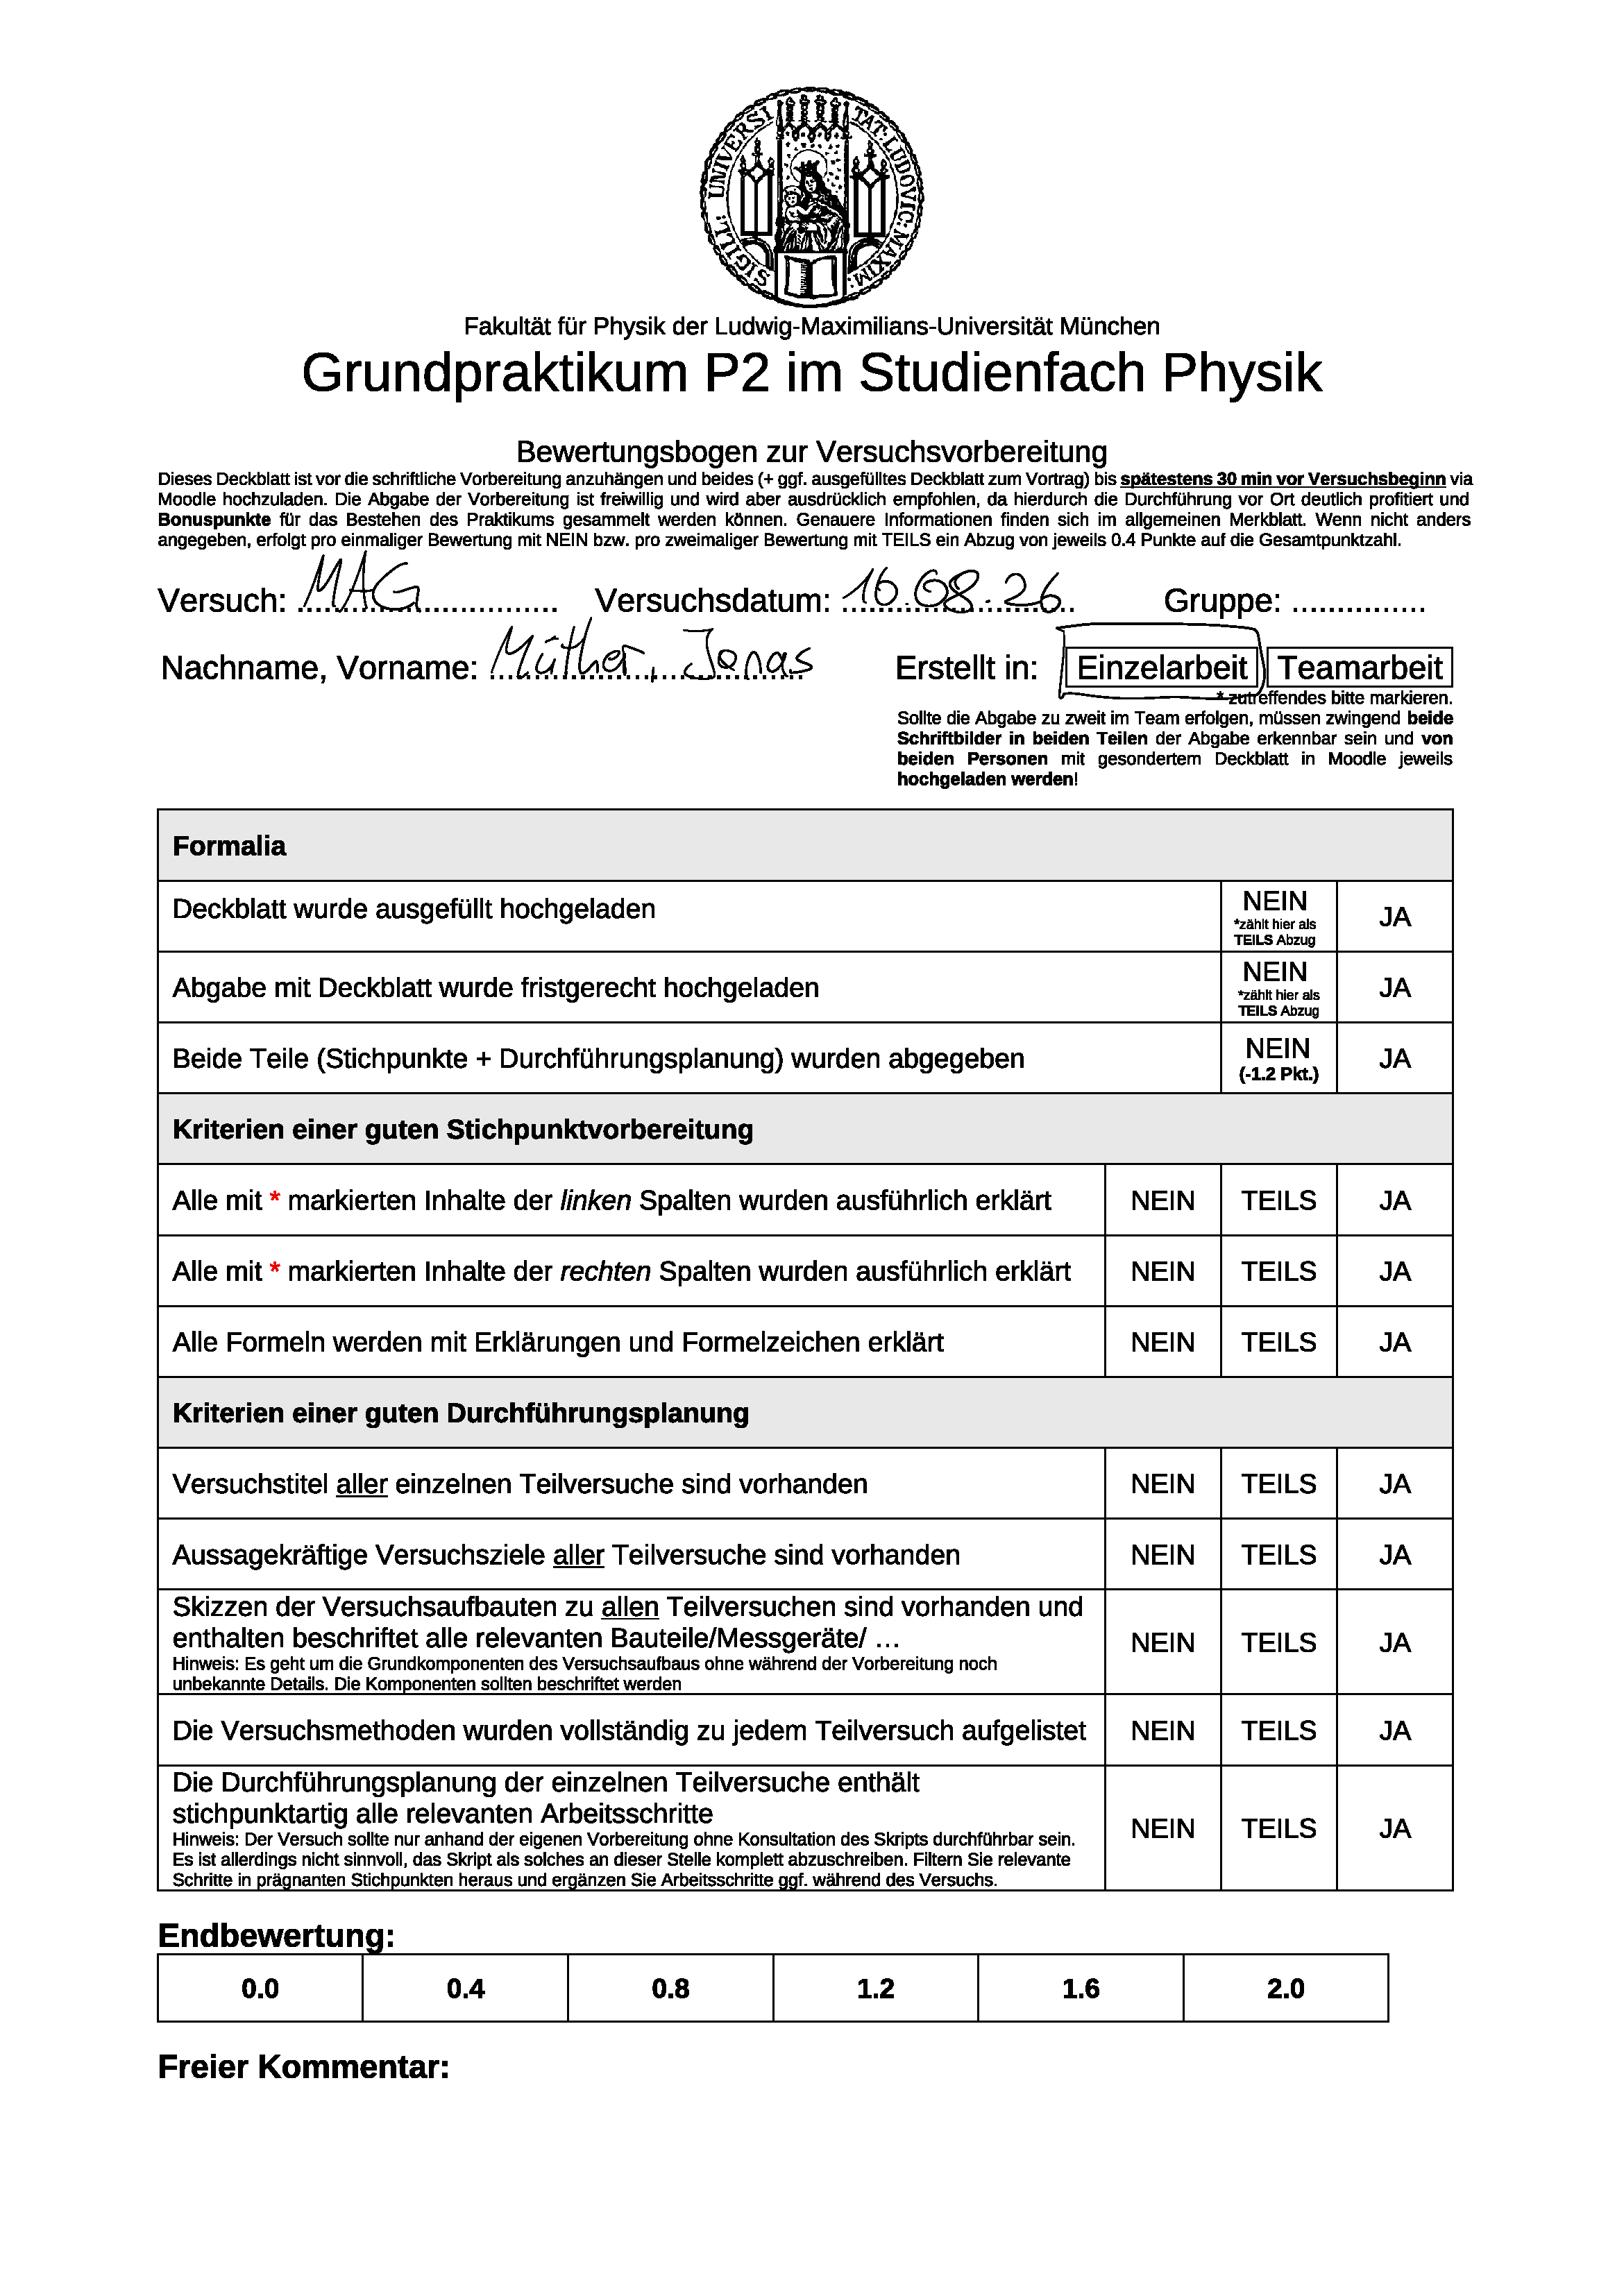
\includepdf[pages=-]{./PDFs/VorbereitungMAG.pdf}

\section{Versuchsprotokoll}
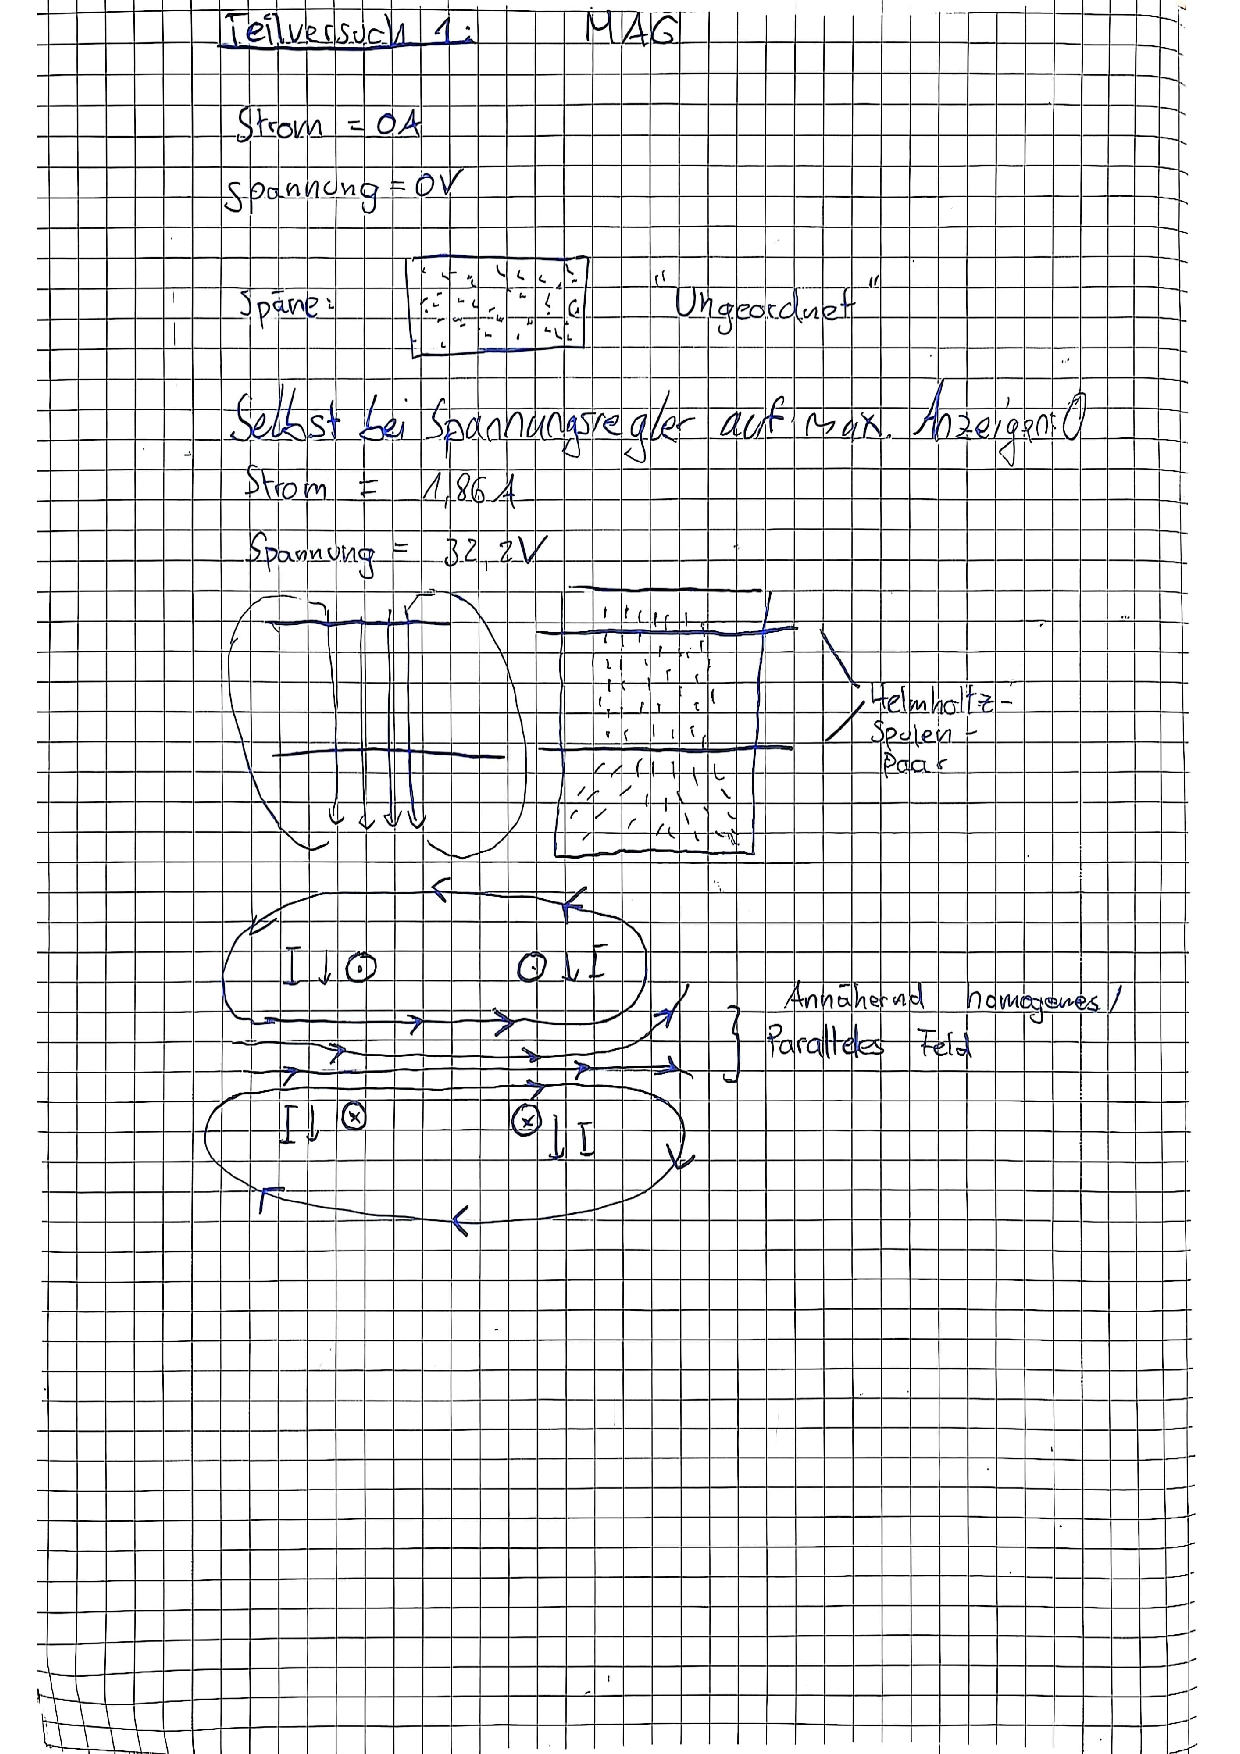
\includepdf[pages=-]{./PDFs/MAGProtokoll.pdf}

\newpage
\chapter{Auswertung}
\newpage
\section{Teilversuch II: Drehmoment des Feldes auf eine stromdurchflossene Spule}
Im zweiten Teilversuch sollte das Drehmoment untersucht werden, dass auf eine stromdurchflossene Spule in einem näherungsweise homogenen Magnetfeld  wirkt.
Hierzu wurden zu verschiedenen Winkeln zwischen Spulenachse und Magnetfeldrichtung der Torsionswinkel eines Drahtes gemessen. Dieser ist proportional zum wirkenden 
Drehmoment.
Das auf die Spule wirkende Drehmoment wird beschrieben durch:
\begin{equation}
    \begin{split}
        M = IAB \sin(\alpha)
    \end{split}
\end{equation}
Wobei $\alpha$ den winkel zwischen der Flächennormalen der Spule und dem Magnetfeld beschreibt. Dieses Drehmoment bewirkt eine Verdrillung des Torsionsdrahts,
die folgendermaßen beschrieben werden kann:
\begin{equation}
    \begin{split}
        M = -D \varphi
    \end{split}
\end{equation}
Setzt man diese Formeln zusammen, erhält man folgende Proportionalität zwischen $\varphi$ und $\sin(\alpha)$:
\begin{equation}
    \varphi = - \frac{IAB}{D} \sin(\alpha)
    \label{eq:phiSinAlphaTheor}
\end{equation}
Das Ziel im Folgenden ist es, diese Proportionalität mithilfe der aufgezeichneten Daten zu überprüfen.
Im Versuch wurde für gegebene $\alpha$ der Winkel des Einstellknopfs ($\beta$) bestimmt. Der Winkel $\varphi$ errechnet sich aus diesen Winkeln wie folgt:
\begin{equation}
    \varphi = \alpha - \beta
\end{equation}
Der Fehler von $\varphi$ berechnet sich folgendermaßen:
\begin{equation}
    \begin{split}
        \Delta \varphi &= \sqrt{\left(\frac{\partial \varphi}{\partial \alpha}\Delta \alpha\right)^2 + \left(\frac{\partial \varphi}{\partial \beta}\Delta \beta\right)^2} \\
                    &= \sqrt{(\Delta \alpha)^2 + (\Delta \beta)^2}
    \end{split}
\end{equation}
Zur Auswertung ist zu beachten, dass während der Versuchsdurchführung ein Winkel $\tilde{\beta}$ gemessen wurde, der noch über einen Anfangsoffset verschoben ist. 
Der tatsächliche Winkel $\beta$ muss also noch folgendermaßen berechnet werden:
\begin{equation}
    \beta = \tilde{\beta} - \beta_0
\end{equation}
In unserem Fall lag der Winkel $\beta_0$ bei $\qty{268.0}{\degree}$
Führt man die beschriebenen Manipulationen mithilfe eines Python Skripts (Siehe \ref{scr:calcAng}) durch, erhält man folgende Werte:
\begin{table}[H]
        \begin{center}
                \begin{tabular}{|c|c|c|}
                        \hline
                        $\alpha$ in $^{\circ}$ & $\beta$ in $^{\circ}$ & $\varphi$ in $^{\circ}$ \\
                        \hline
                        $0.0 \pm 2.0$ & $0.0 \pm 1.0$ & $0.0 \pm 2.3$ \\
                        \hline
                        $10.0 \pm 2.0$ & $18.0 \pm 1.0$ & $-8.0 \pm 2.3$ \\
                        \hline
                        $20.0 \pm 2.0$ & $39.0 \pm 1.0$ & $-19.0 \pm 2.3$ \\
                        \hline
                        $30.0 \pm 2.0$ & $54.5 \pm 1.0$ & $-24.5 \pm 2.3$ \\
                        \hline
                        $40.0 \pm 2.0$ & $72.0 \pm 1.0$ & $-32.0 \pm 2.3$ \\
                        \hline
                        $50.0 \pm 2.0$ & $88.0 \pm 1.0$ & $-38.0 \pm 2.3$ \\
                        \hline
                        $60.0 \pm 2.0$ & $102.5 \pm 1.0$ & $-42.5 \pm 2.3$ \\
                        \hline
                        $70.0 \pm 2.0$ & $116.0 \pm 1.0$ & $-46.0 \pm 2.3$ \\
                        \hline
                        $80.0 \pm 2.0$ & $128.0 \pm 1.0$ & $-48.0 \pm 2.3$ \\
                        \hline
                        $90.0 \pm 2.0$ & $139.5 \pm 1.0$ & $-49.5 \pm 2.3$ \\
                        \hline
                \end{tabular}
        \end{center}
        \caption{Berechnete Winkel}
        \label{tab:angles}
\end{table}
\noindent
Wir überprüfen nun die Proportionalität zwischen $\varphi$ und $\sin(\alpha)$, indem wir die Werte der Tabelle \ref{tab:angles} in ein Diagramm Plotten.
Per Konvention entscheiden wir uns hier, $-\varphi$ gegenüber $\sin(\alpha)$ zu plotten. Die Steigung der theoretisch vorhergesagten Ursprungsgeraden entspricht dann: $m = (IAB)/D$.
Fittet man eine Ausgleichsgerade an die Messwerte (\ref{scr:phiSinAlpha}), erhält man dieses Diagramm:
\begin{figure}[H]
    \centering
    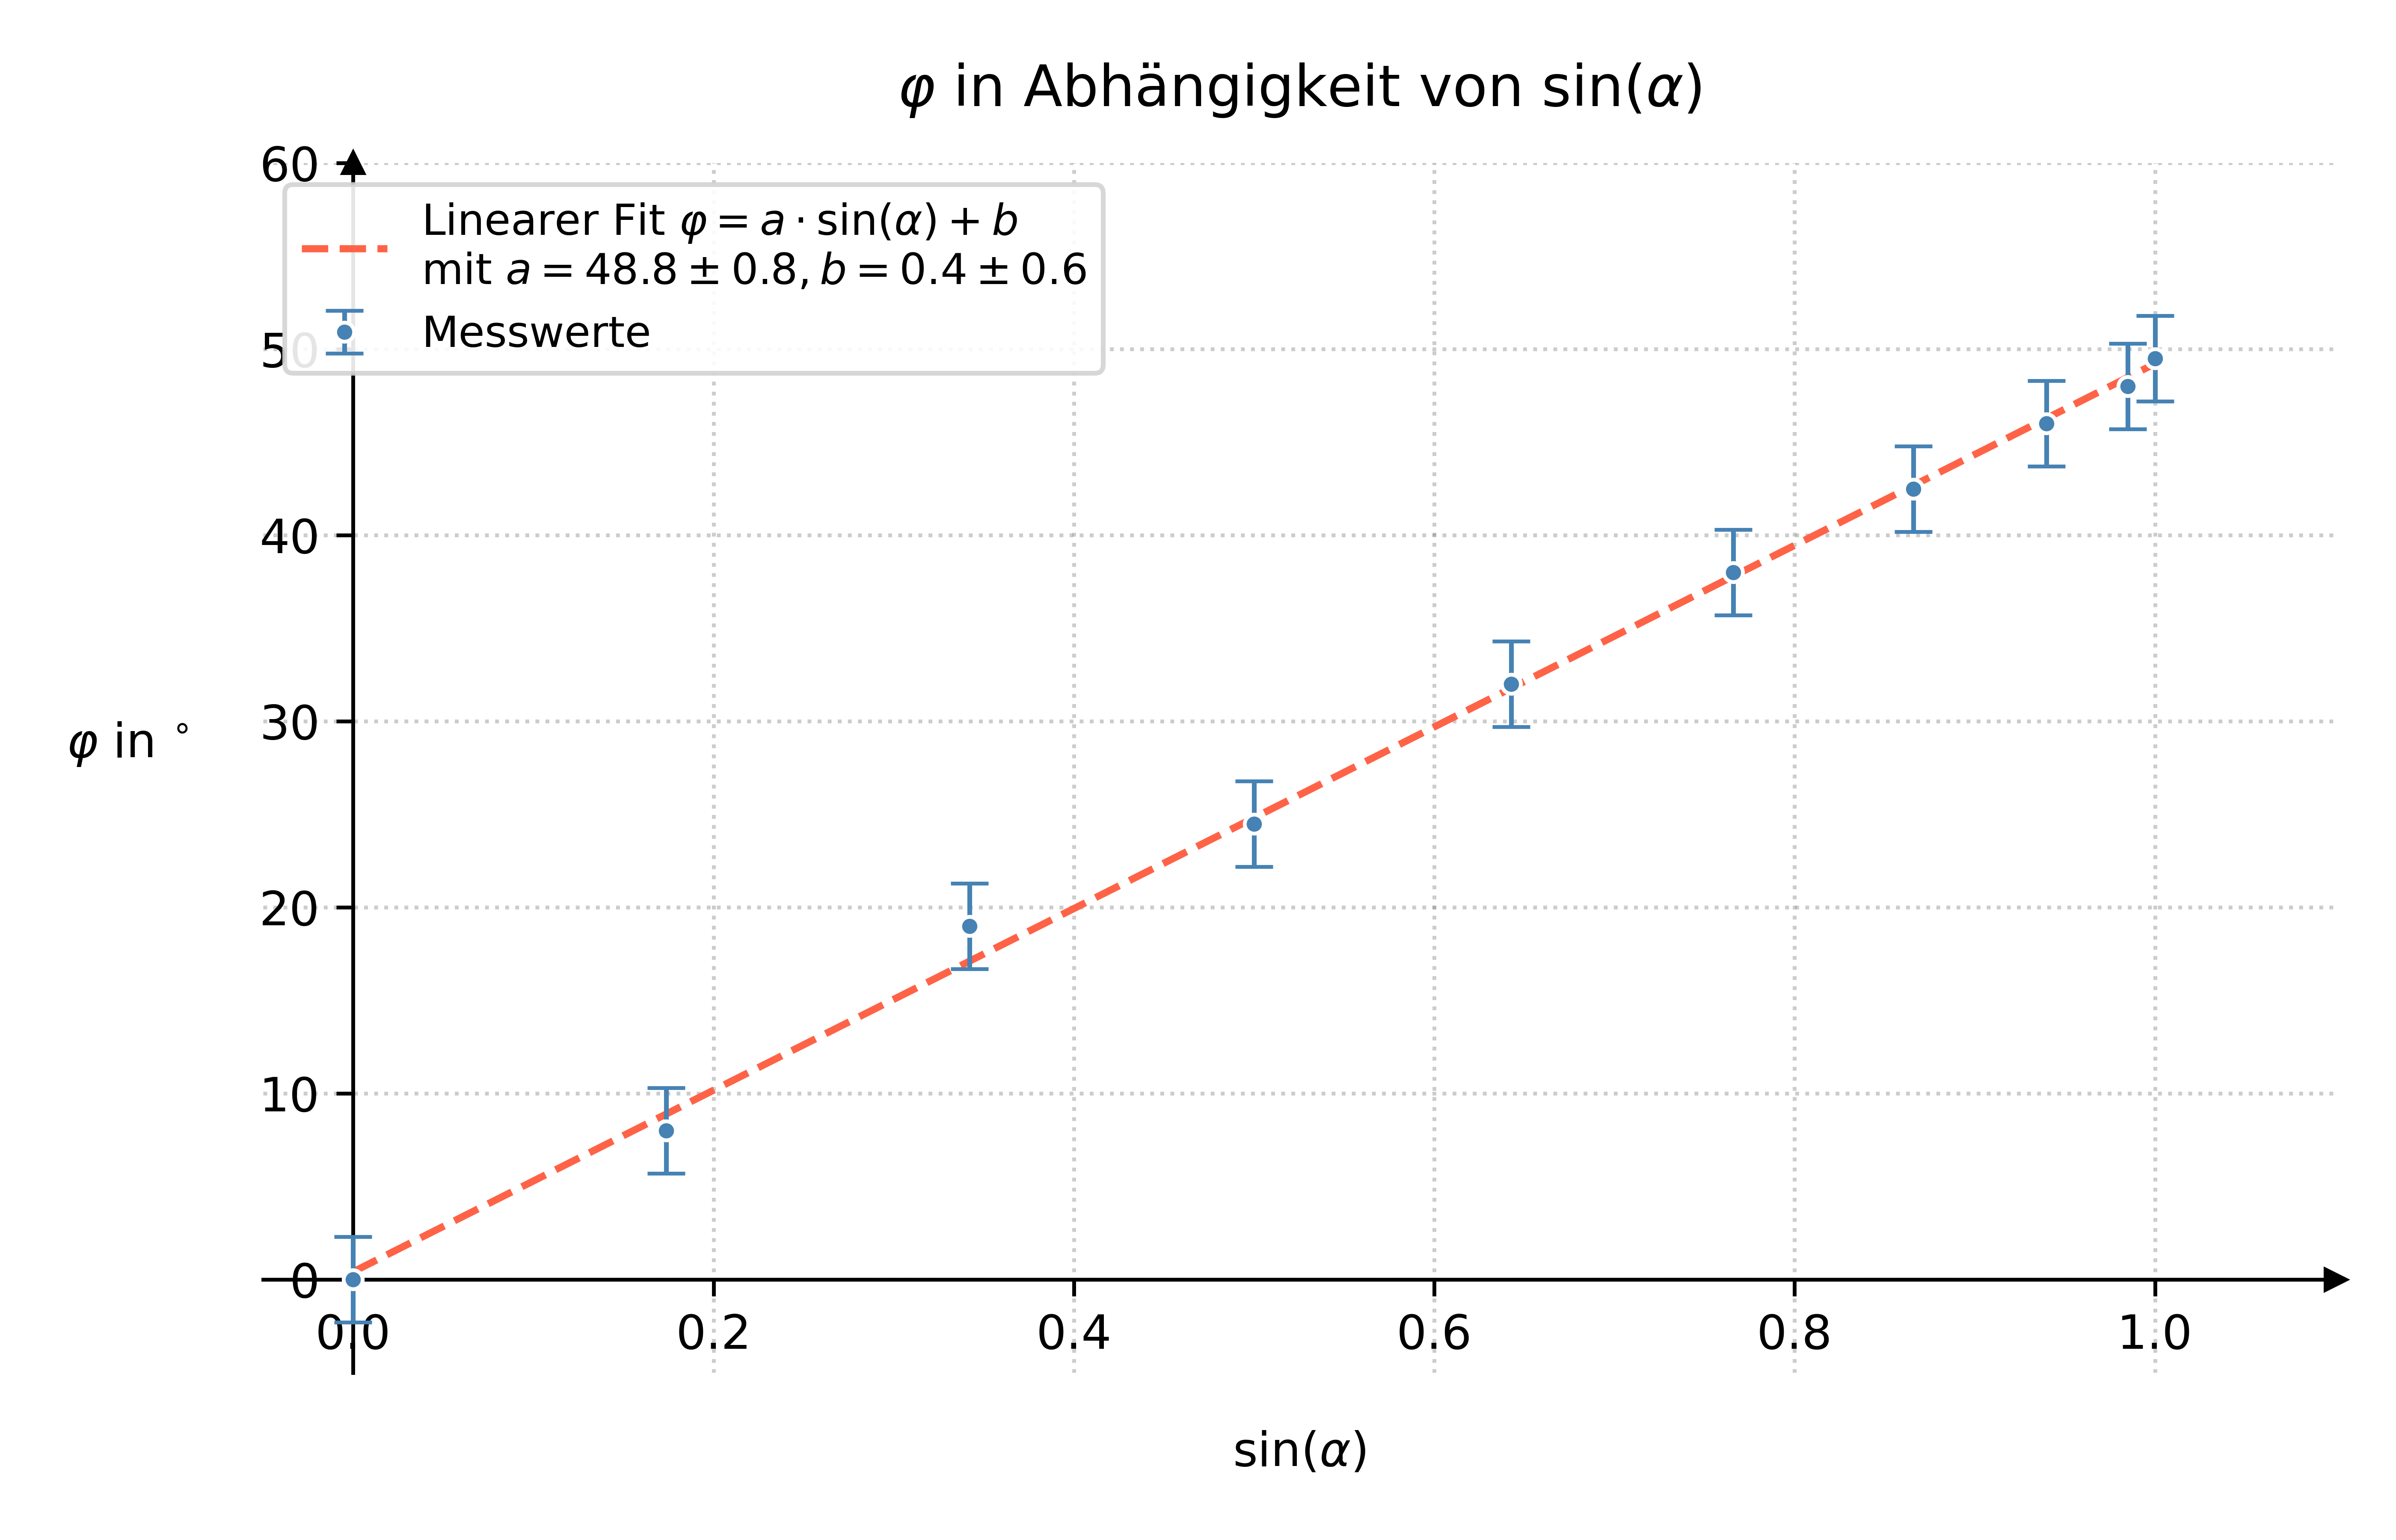
\includegraphics[width=1\textwidth]{./Images/PhiSinAlpha.png}
    \caption{$\varphi(\sin(\alpha))$-Diagramm}
    \label{fig:PhiSinAlpha}
\end{figure}
Am Parameter $b = (0.4 \pm 0.6)^{\circ}$ ist erkennbar, dass die Messwerte im Rahmen der Unsicherheit tatsächlich auf einer durch den Ursprung verlaufenden Gerade liegen,
da $b$ den Ordinatenabschnitt der Gerade angibt und der Wert $b* = 0$ für den es sich um eine Ursprungsgerade handelt innerhalb der Unsicherheitsgrenzen liegt.
Damit ist die theoretische Vorhersage (\ref{eq:phiSinAlphaTheor}) experimentell bestätigt.
Der Proportionalitätsfaktor hierzu ist gegeben durch:
\begin{equation}
    \begin{split}
        \frac{IAB}{D} = (48.8 \pm 0.8)^{\circ}
    \end{split}
\end{equation}
\newpage
\section{Teilversuch III: Induktion durch Drehen einer Spule im Magnetfeld}
In Teilversuch III wurde die Induktion durch das Rotieren einer Spule im näherungsweise homogenen Magnetfeld eines Helmholtz Spulenpaars untersucht.
Hierzu wurde mithilfe eines XY/t-Schreibers ein $U_{\mathrm{ind}}(t)$-Diagramm (Abb. \ref{fig:UIndtDiagrammBewegungsinduktion}) aufgezeichnet.
Aus diesem Diagramm konnten folgende Spannungsamplituden abgelesen werden:
\begin{table}[H]
    \centering
    \caption{Spannungsamplituden der Bewegungsinduktion}
    \label{tab:AmpBewInd}
    \begin{tabular}{c c}
        \hline
        Index das Extremums & $\hat{U}_i$ in \si{V}\\
        \hline
        1 &  1.095\\
        2 &  1.105\\
        3 &  1.055\\
        4 &  1.125\\
        5 &  1.085\\
        6 &  1.125\\
        7 &  1.080\\
        8 &  1.125\\
        9 &  1.120\\
        10 &  1.130\\
        11 &  1.095\\
        12 &  1.135\\
        13 &  1.115\\
        14 &  1.115\\
        15 &  1.080\\
        16 &  1.115
    \end{tabular}
\end{table}
\noindent
Zunächst berechnen wir aus diesen Werten den Mittelwert und dessen statistischen Fehler. Dies geschieht mithilfe des Python Scripts \ref{scr:meanAndError}.
Die Berechnung des Fehlers erfolgt dabei nach folgender Formel:
\begin{equation}
    s_{\bar{U}} = \frac{s_{U}}{\sqrt{n}}
\end{equation}
Wobei $n$ die Anzahl der Messpunkte ist und die Standardabweichung $s_U$ durch die empirische Streuung gegeben ist:
\begin{equation}
    \begin{split}
        s_U = \sqrt{\frac{1}{n-1}\sum_{i=1}^{n} (U_i - \bar{U})^2}
    \end{split}
\end{equation}
Bei Durchführung der Berechnungen erhält man folgendes Ergebnis für den Mittelwert der Spannungsamplitude sowie dessen Fehler: 
\begin{equation}
    \bar{\hat{U}}_{\mathrm{ind}} = 1.106 \pm 0.006
\end{equation}
Hierbei handelt es sich um die korrekte Berechnung des Fehlers, da dieser aus der statistischen Streuung der gemessenen Spannungsamplituden hervorgeht, weshalb sich 
der Fehler aus der Standardabweichung wie oben beschrieben berechnet.
\begin{figure}[H]
    \centering
    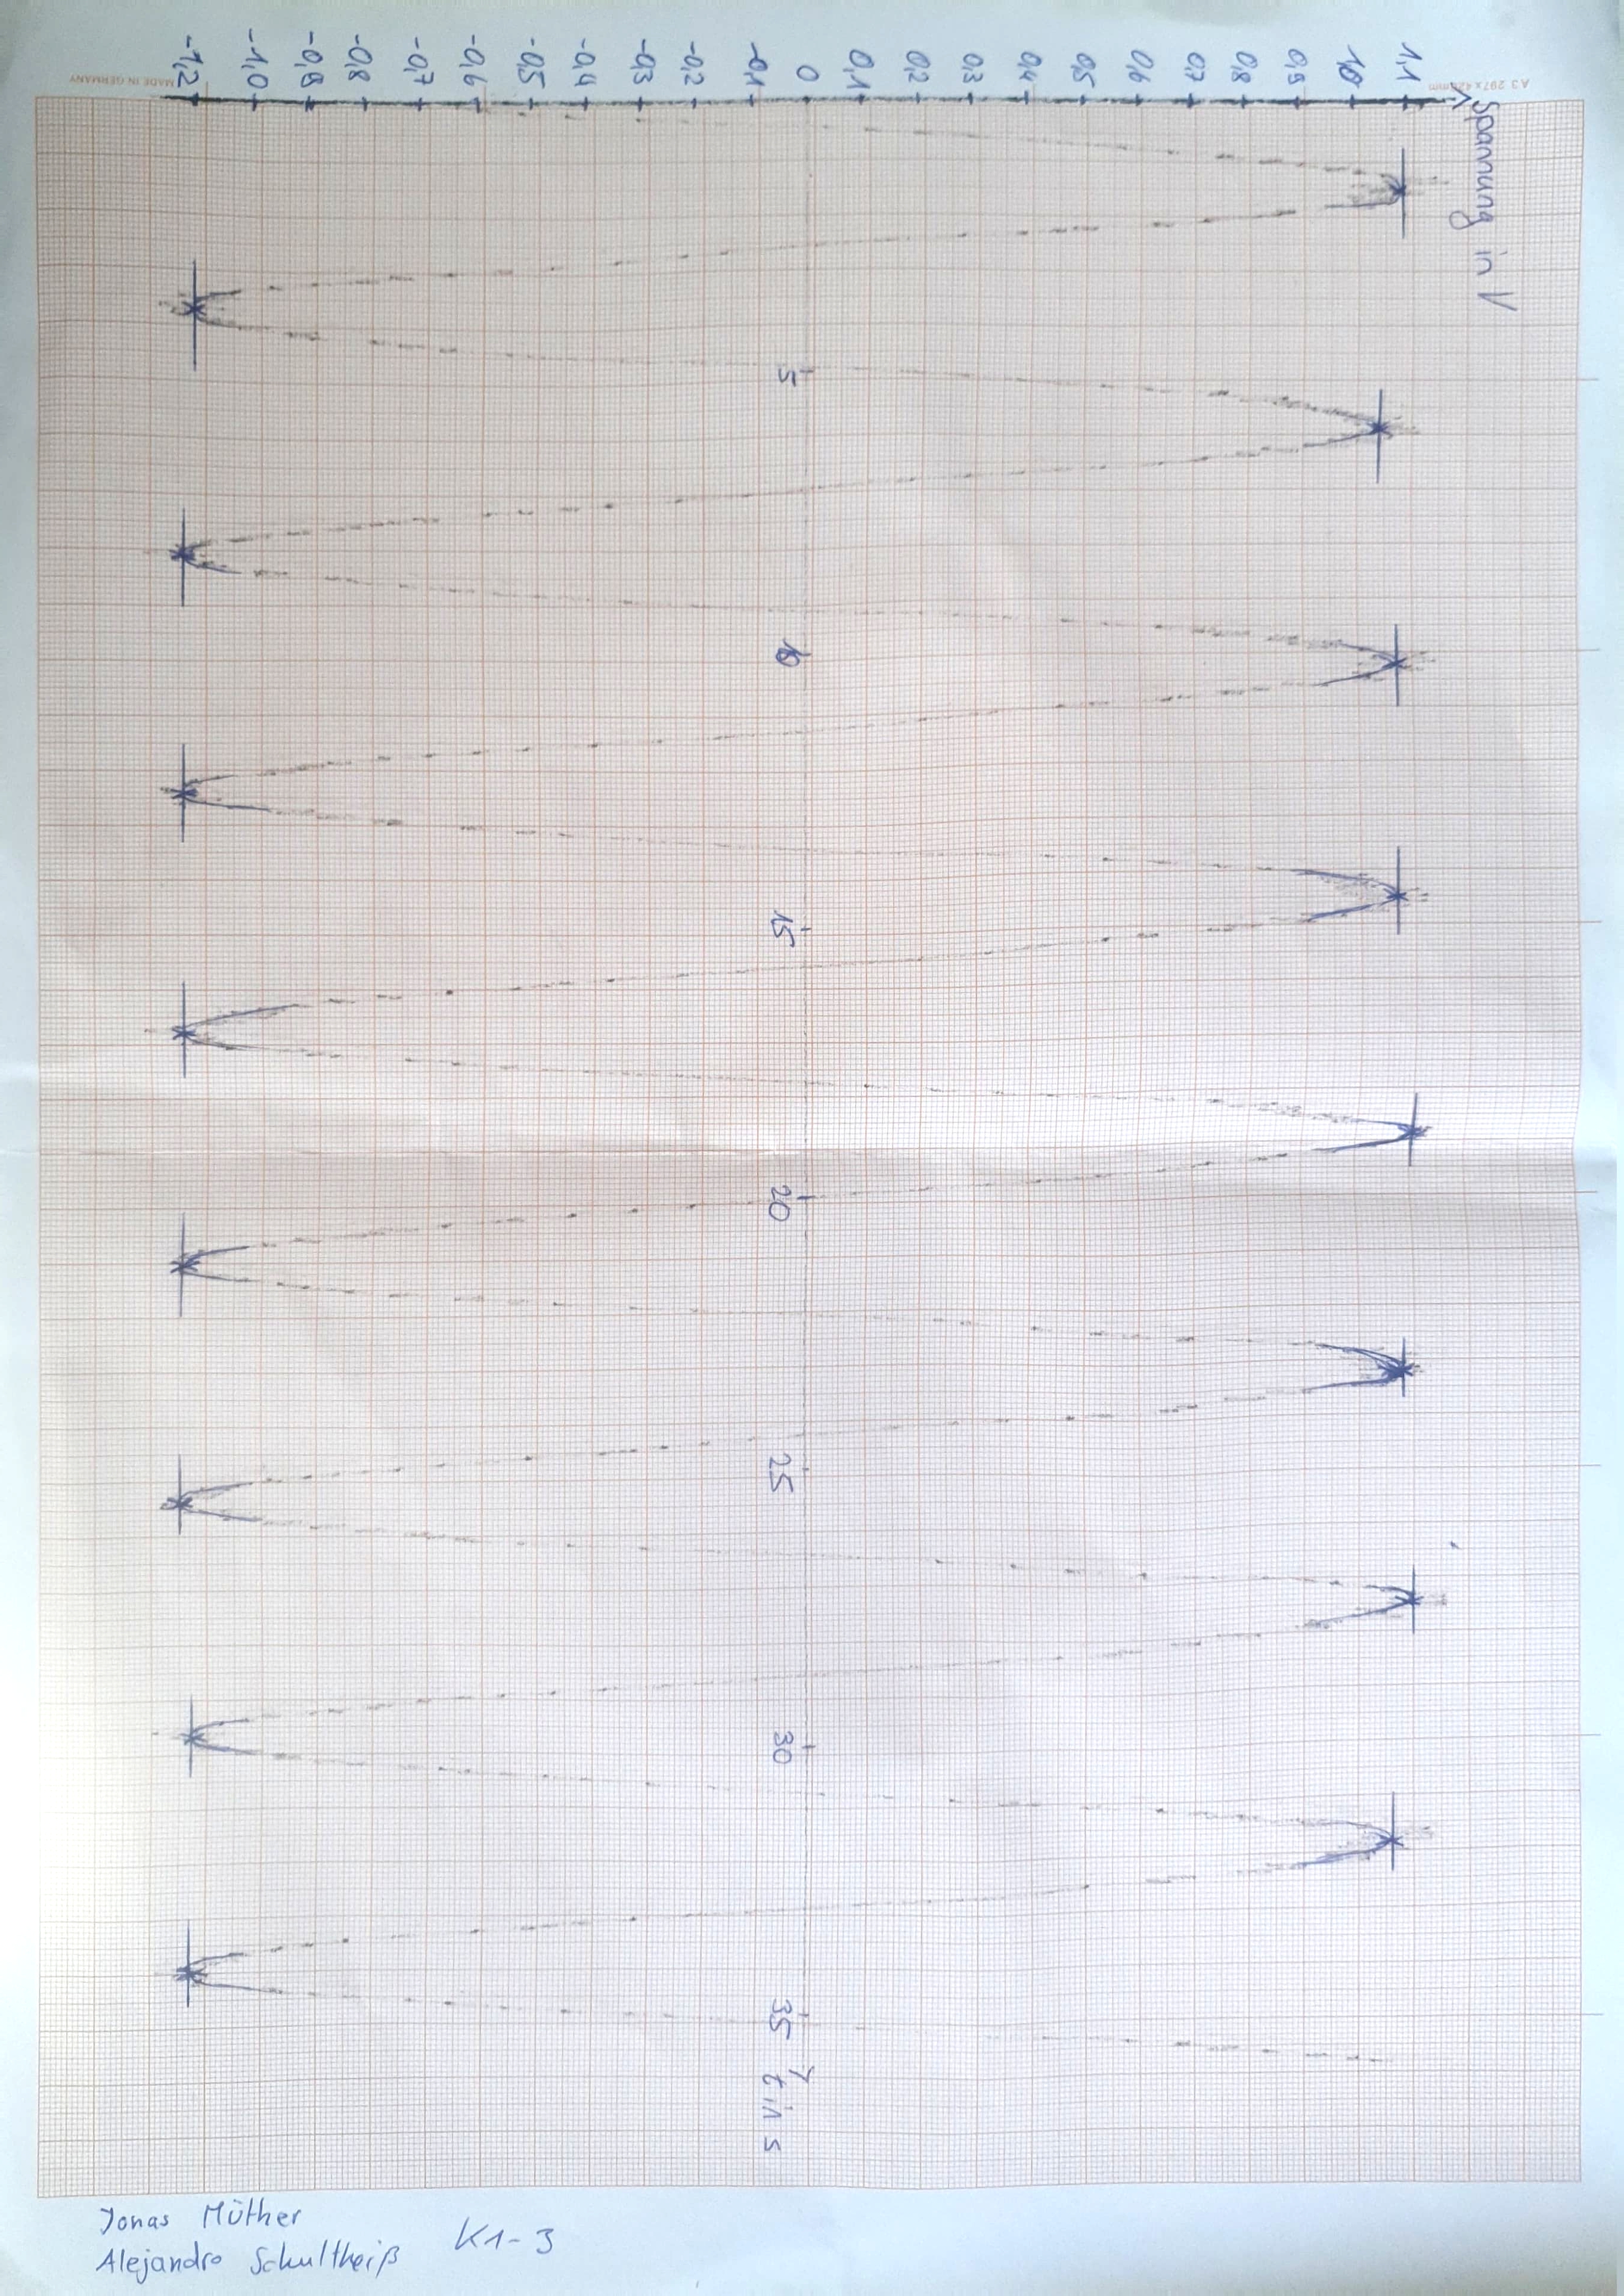
\includegraphics[width=.9\textwidth]{./Images/UIndtDiagrammBewegungsinduktion.jpg}
    \caption{$U_{ind}(t)$-Diagramm einer rotierenden Spule im homogenen Magnetfeld}
    \label{fig:UIndtDiagrammBewegungsinduktion}
\end{figure}
\noindent
Aus den experimentellen Daten kann nun der Betrag der Magnetischen Flussdichte ($\left\lvert\vec{B}\right\rvert$) errechnet werden. 
Für die Spule Induktionsspannung einer rotierenden Spule gilt:
\begin{equation}
    U_{\mathrm{ind}} = NBA\omega\sin(\omega t) = \hat{U}_{\mathrm{ind}} \sin(\omega t)
\end{equation}
Daraus folgt:
\begin{equation}
    B = \frac{\hat{U}_{\mathrm{ind}}}{NA\omega}
    \label{eq:BExp}
\end{equation}
Dabei werden $A = \qty{23.5e-4}{\meter \squared}$ und $N = 82800$ als fehlerfrei angegeben.
Die Winkelgeschwindigkeit errechnet sich aus der Rotationsfrequenz des Motors. Diese ist angegeben als $f_0 = \qty{16.6}{min^{-1}}$ (bei $\qty{60}{Hz}$ Netzfrequenz).
Da das Stromnetz in Deutschland nur eine Frequenz von $50 \si{Hz}$ hat und die Rotationsfrequenz proportional zur Frequenz der Spannungsversorgung ist, 
ergibt sich folgendes für die Winkelgeschwindigkeit:
\begin{equation}
    \begin{split}
        \omega  &= 2 \pi f \\
                &= 2 \pi f_0 \cdot \frac{50}{60} \\
                &= 2 \pi \cdot 16.6 \si{min^{-1}} \cdot \frac{\si{min}}{60 \si{s}} \cdot \frac{50}{60} \\
                &= 1.449 \si{\per \second}
    \end{split}
\end{equation}
Einsetzen dieser Werte und $\bar{\hat{U}}_{\mathrm{ind}}$ in \ref{eq:BExp} ergibt:
\begin{equation}
    \bar{B} = \qty{3.923}{mT}
\end{equation}
Die Unsicherheit dieses Wertes ergibt sich durch:
\begin{equation}
    \begin{split}
        \Delta B &= \frac{\partial B}{\partial \hat{U}_{\mathrm{ind}}} \cdot \Delta \hat{U}_{\mathrm{ind}} \\
                    &= \frac{\Delta \hat{U}_{\mathrm{ind}}}{NA\omega} \\
                    &= \qty{0.022e-3}{mT}
    \end{split}
\end{equation}
Die experimentell bestimmte Flussdichte liegt also bei:
\begin{equation}
    \boxed{B_{\mathrm{exp}} = (3.923 \pm 0.022) \si{mT}}
\end{equation}
Die magnetische Flussdichte in der Mitte eines Helmholtz Spulenpaars kann auch theoretisch aus den geometrischen Eigenschaften der Spule und dem durch diese fließenden
elektrischen Strom berechnet werden. Hierzu gilt folgender Zusammenhang:.
\begin{equation}
    B_{\mathrm{theo}} = \mu_0 (4/5)^{\frac{3}{2}} \cdot \frac{NI}{R}
    \label{eq:BTheoHelmh}
\end{equation}
Die Windungszahl der Helmholtzspule ist gegeben durch $N = 528$.
Die Stromstärke wurde mithilfe eines Multimeters bestimmt. Der abgelesene Wert lag bei $\bar{I} = 1.119 \si{\ampere}$. In diesem Messbereich liegt der Fehler des Multimeters bei
$\Delta I = 1.0 \% I + 3$.
Demzufolge liegt der mithilfe des gemessene Strom bei:
\begin{equation}
    I = (1.119 \pm 0.015) A
\end{equation}
Zur Berechnung des Radius wurden Innen- und Außendurchmesser der Spule gemessen ($D = (30.70 \pm 0.010) \si{cm}$, $d = (25.10 \pm 0.010) \si{cm}$). 
Der effektive Durchmesser der Spule beträgt damit:
\begin{equation}
    \begin{split}
        D_{\mathrm{eff}}    &= \frac{D + d}{2} \\
                            &= (0.2790 \pm 0.0010) \si{m}
    \end{split}
\end{equation}
Daraus folgt der Radius:
\begin{equation}
    R = \frac{D}{2} = (0.1395 \pm 0.0005) \si{m}
\end{equation}
Setzt man diese Werte in Formel \ref{eq:BTheoHelmh} ein, erhält man:
\begin{equation}
    \bar{B}_{\mathrm{theo}} = \qty{3.8083}{mT}
\end{equation}
Die Unsicherheit dieses Messwerts ist gegeben durch:
\begin{equation}
    \begin{split}
        \Delta B_{\mathrm{theo}} &= \sqrt{\left(\frac{\partial B}{\partial R}\cdot \Delta R\right)^2 + \left(\frac{\partial B}{\partial I} \cdot \Delta I\right)^2} \\
                                 &= B_{\mathrm{theo}} \sqrt{\left(\frac{\Delta R}{R}\right)^2 + \left(\frac{\Delta I}{I}\right)^2} \\
                                 &= \qty{0.06}{mT}
    \end{split}
\end{equation}
Das Endergebnis für die theoretisch bestimmte Flussdichte liegt damit bei:
\begin{equation}
    \begin{split}
        \boxed{B_{\mathrm{theo}} = (3.81 \pm 0.06) \si{mT}}
    \end{split}
\end{equation}
Vergleicht man den theoretisch berechneten und den experimentell bestimmten Wert für die Flussdichte, fällt auf, dass die im Rahmen der Messunsicherheit nicht 
übereinstimmen. Im Rahmen eines $3\sigma$-Intervalls sind die Werte allerdings miteinander verträglich. Mögliche Fehler in der experimentellen Bestimmung könnten
beispielsweise dadurch entstehen, dass das Feld der Helmholtzspule nicht perfekt homogen ist, durch einen nicht perfekt mit der angegebenen Frequenz drehenden Motor 
oder durch die Ungenauigkeit des Schreibers. Diese Werte wurden in der Auswertung als fahlerfreie Daten angenommen, was in der Realität natürlich niemals der Fall
sein kann.
\newpage
\section{Teilversuch IV: }
\noindent
In diesem Teilversuch wurde die Induktionsspule nicht bewegt, während das Magnetfeld
der Helmholtzspule zeitlich verändert wurde. Hierzu wurde ein dreieckförmiger
Feldstrom mithilfe des Funktionengenerators angelegt. Mit dem XY/t-Schreiber wurden sowohl der zeitliche Verlauf des
Feldstroms als auch die an der Induktionsspule auftretende Induktionsspannung
aufgezeichnet.
\noindent
Gemäß dem Induktionsgesetz gilt

\begin{equation}
U_{\mathrm{ind}}
=
-N_{\mathrm I}A_{\mathrm I}
\frac{\mathrm dB}{\mathrm dt}.
\end{equation}
\noindent
Da das Magnetfeld der Helmholtzspule bei unveränderter Geometrie proportional zum
Feldstrom ist,

\begin{equation}
B\propto I,
\end{equation}
\noindent
folgt

\begin{equation}
U_{\mathrm{ind}}
\propto
-\frac{\mathrm dI}{\mathrm dt}.
\end{equation}
\noindent
Bei einem dreieckförmigen Feldstrom ist die zeitliche Änderung des Stroms innerhalb
einer Halbperiode näherungsweise konstant. Entsprechend wird also innerhalb einer
Halbperiode eine näherungsweise konstante Induktionsspannung erwartet.

\subsection{Skalierung des Schreiberdiagramms}
\noindent
Die Zeitablenkung des Schreibers betrug

\begin{equation}
1\,\mathrm{s/cm}.
\end{equation}
\noindent
Damit gilt für die Zeitachse

\begin{equation}
\boxed{
1\,\mathrm{cm}
\;\widehat{=}\;
1\,\mathrm{s}
}.
\end{equation}
\noindent
Die vertikale Komponente des Schreibers betrug

\begin{equation}
20\,\mathrm{mV/cm}.
\end{equation}
\noindent
Der Feldstrom wurde über den Spannungsabfall an einem Messwiderstand

\begin{equation}
R=(0{,}150\pm0{,}002)\,\Omega
\end{equation}
\noindent
bestimmt. Nach dem Ohmschen Gesetz gilt

\begin{equation}
I=\frac{U_R}{R}.
\end{equation}
\noindent
Eine vertikale Auslenkung von einem Zentimeter entspricht daher einem Feldstrom von

\begin{align}
I_{\mathrm{1\,cm}}
&=
\frac{20\,\mathrm{mV}}{0{,}150\,\Omega} \\
&=
0{,}13333\ldots\,\mathrm{A}.
\end{align}
\noindent
Somit wurde die Ordinate der Feldstromkurven mit

\begin{equation}
\boxed{
1\,\mathrm{cm}
\;\widehat{=}\;
0{,}1333\,\mathrm{A}
}
\end{equation}
\noindent
skaliert. Für die Induktionsspannung gilt entsprechend

\begin{equation}
\boxed{
1\,\mathrm{cm}
\;\widehat{=}\;
20\,\mathrm{mV}
}.
\end{equation}

\begin{figure}[htbp]
    \centering
    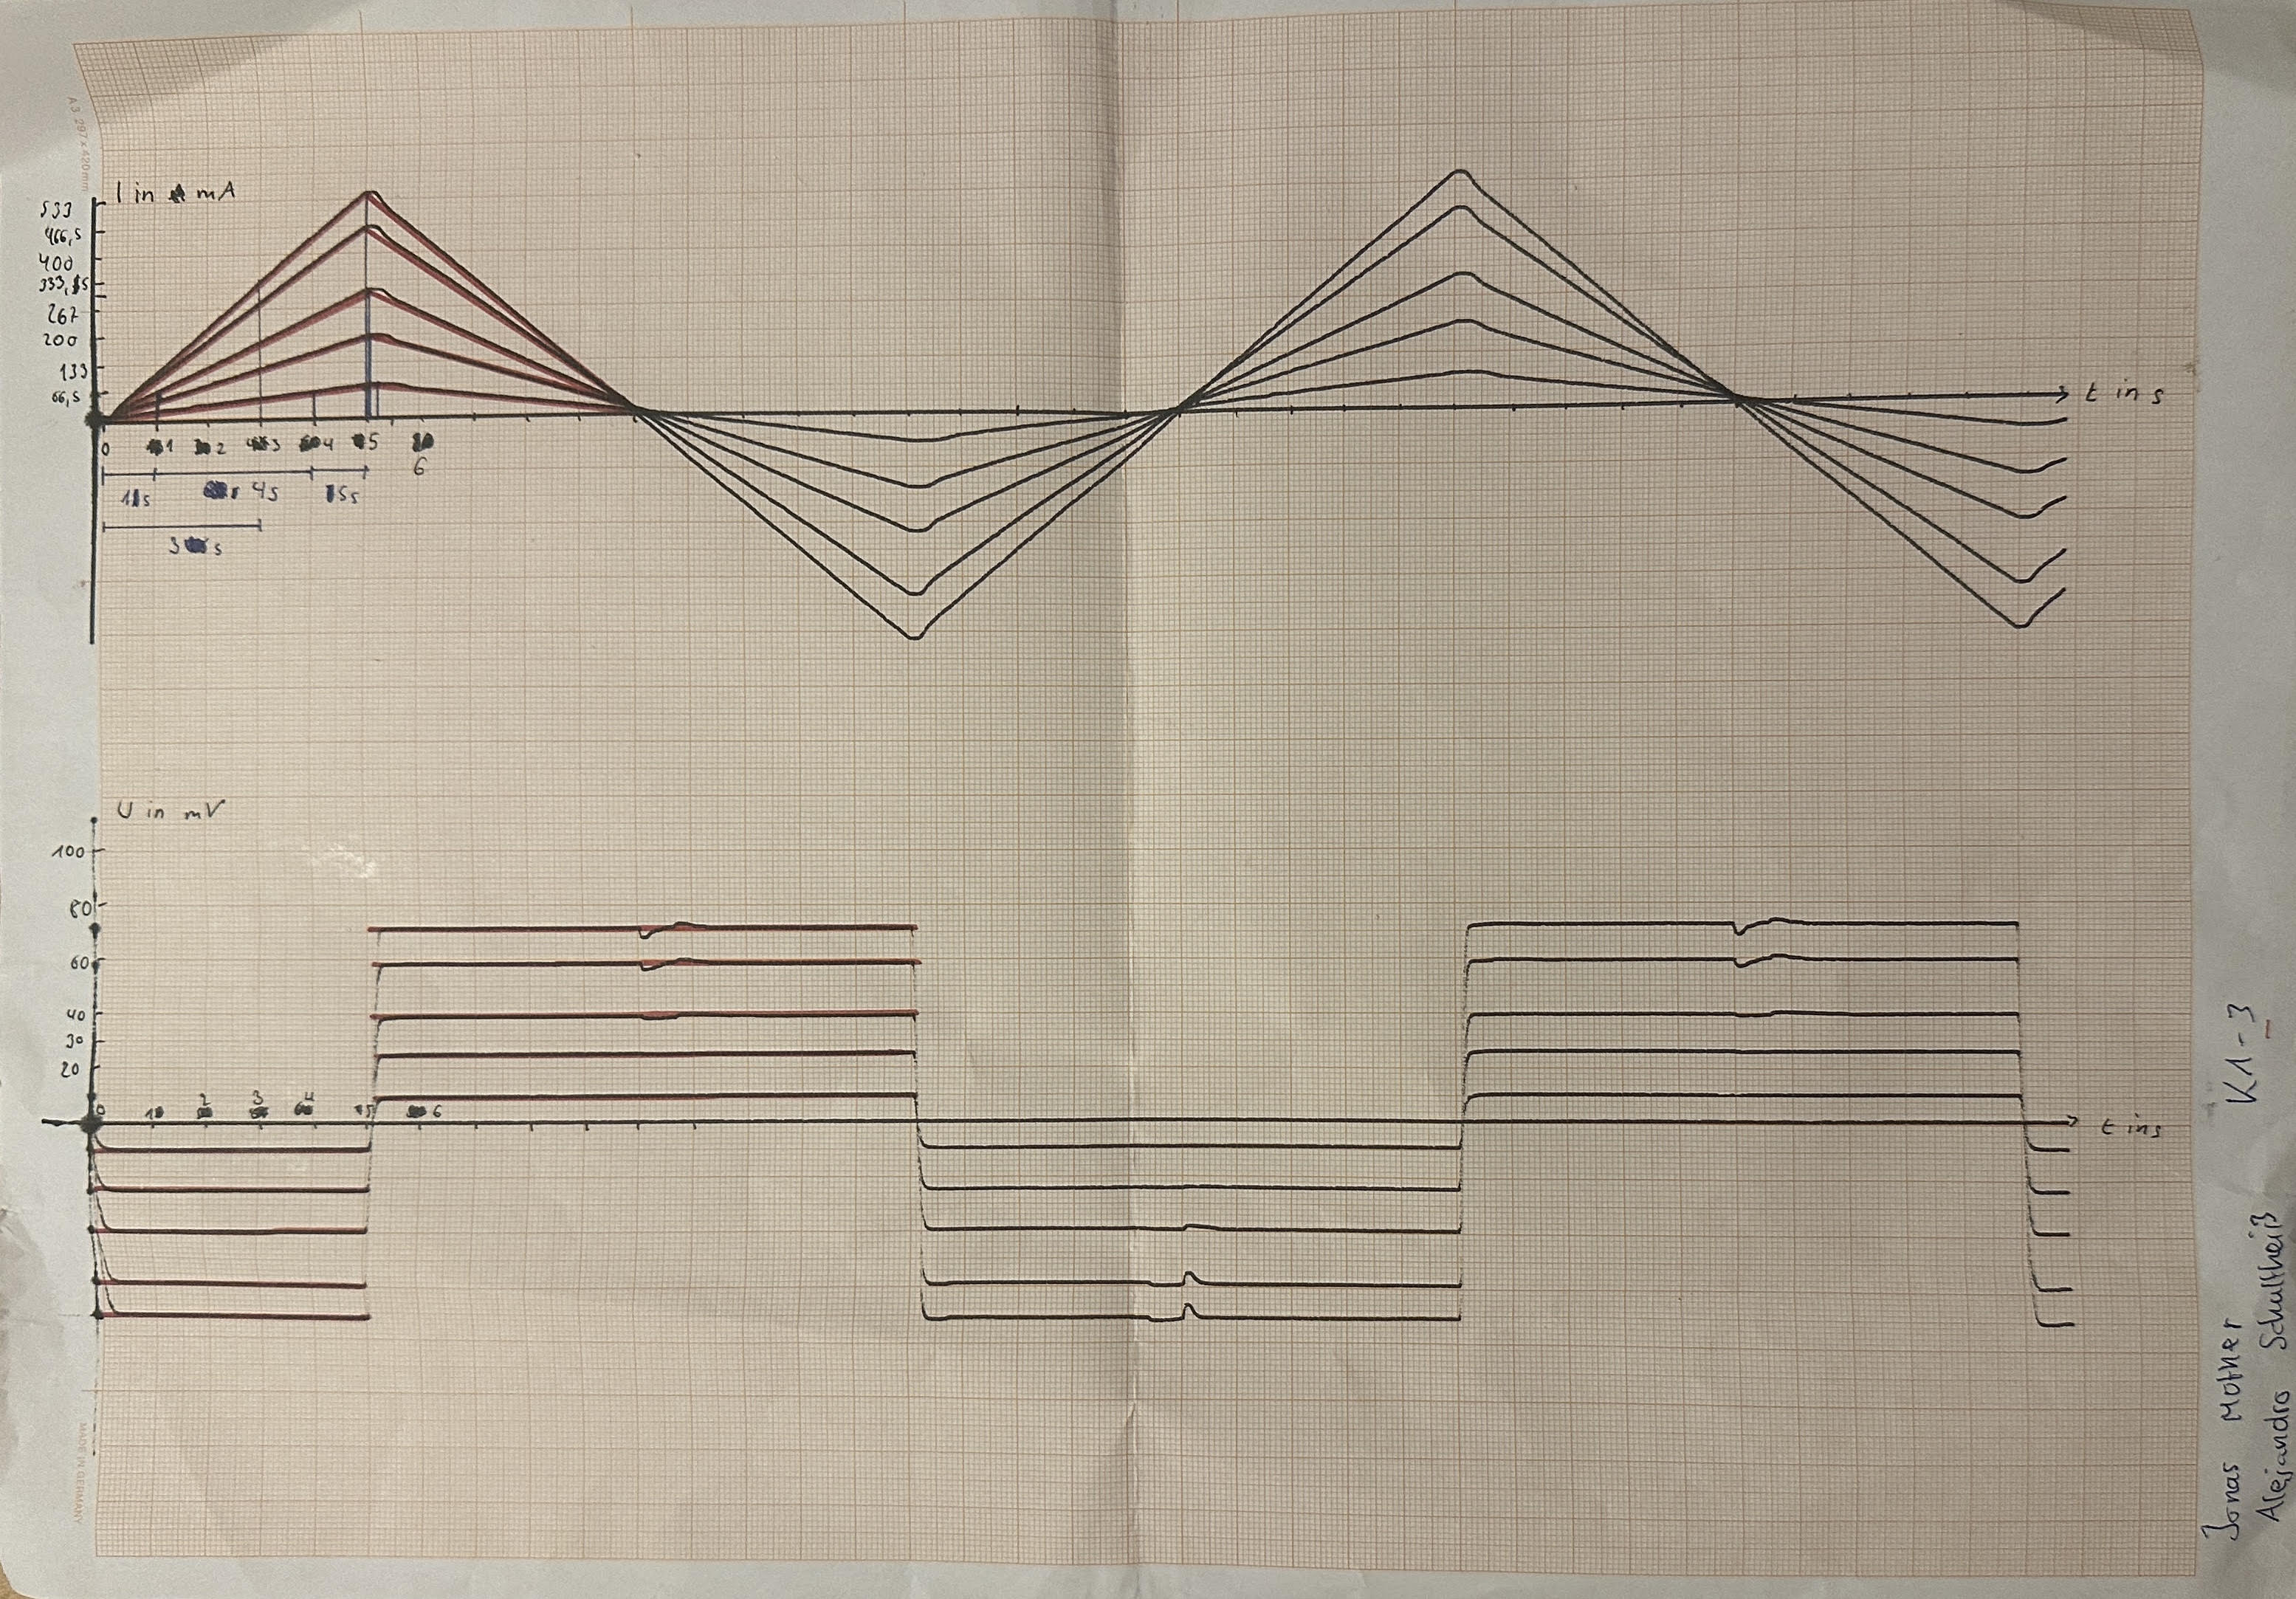
\includegraphics[width=0.8\textwidth]{Images/unnamed-4.jpg}
    \caption{Mit dem XY/t-Schreiber aufgezeichnete Verläufe des Feldstroms
    und der induzierten Spannung.}
    \label{fig:schreiber_tv4}
\end{figure}


\subsection{Ableseunsicherheiten}
\noindent
Da die benötigten Größen von Hand aus dem Schreiberdiagramm auf Millimeterpapier
abgelesen wurden, und kein Mittelwert genutzt wird, wurde für die Bestimmung einer Strecke eine Ableseunsicherheit von

\begin{equation}
\Delta l
=
0{,}5\,\mathrm{mm}
=
0{,}05\,\mathrm{cm}
\end{equation}
\noindent
angenommen.
\noindent
Mit der Zeitablenkung von $1\,\mathrm{s/cm}$ ergibt sich

\begin{equation}
\Delta t
=
1\,\mathrm{\frac{s}{cm}}
\cdot0{,}05\,\mathrm{cm}
=
0{,}05\,\mathrm{s}.
\end{equation}
\noindent
Für eine vertikal abgelesene Spannung folgt

\begin{equation}
\Delta U
=
20\,\mathrm{\frac{mV}{cm}}
\cdot0{,}05\,\mathrm{cm}
=
1{,}0\,\mathrm{mV}.
\end{equation}
\noindent
Bei der Bestimmung des Feldstroms muss zusätzlich die Unsicherheit des
Messwiderstands berücksichtigt werden. Für eine Stromdifferenz $\Delta I$ ergibt
sich daher

\begin{equation}
\delta(\Delta I)
=
\sqrt{
\left(
\frac{1{,}0\,\mathrm{mV}}{R}
\right)^2
+
\left(
\Delta I\frac{\Delta R}{R}
\right)^2
}.
\end{equation}


\subsection{Bestimmung der Feldstromsteigungen}
\noindent
Für jede der fünf aufgenommenen Feldstromkurven wurde in der ausgewählten
Halbperiode eine rote Ausgleichsgerade durch den näherungsweise linearen Verlauf gelegt.
Der Betrag der Steigung ergibt sich aus

\begin{equation}
\left|
\frac{\mathrm dI}{\mathrm dt}
\right|
\approx
\frac{\Delta I}{\Delta t}.
\end{equation}
\noindent
Die Unsicherheit der Steigung wurde mit Gaußscher Unsicherheitsfortpflanzung
bestimmt:

\begin{equation}
\delta\left(
\frac{\Delta I}{\Delta t}
\right)
=
\frac{\Delta I}{\Delta t}
\sqrt{
\left(
\frac{\delta(\Delta I)}{\Delta I}
\right)^2
+
\left(
\frac{\delta t}{\Delta t}
\right)^2
}.
\end{equation}
\noindent
Für die erste Kurve ergibt sich beispielsweise

\begin{align}
\left|
\frac{\mathrm dI}{\mathrm dt}
\right|_1
&=
\frac{66{,}5\,\mathrm{mA}}{4\,\mathrm{s}}\\
&=
16{,}625\,\mathrm{\frac{mA}{s}}.
\end{align}
\noindent
Unter Berücksichtigung der Unsicherheiten folgt

\begin{equation}
\boxed{
\left|
\frac{\mathrm dI}{\mathrm dt}
\right|_1
=
(16{,}6\pm1{,}7)\,
\mathrm{\frac{mA}{s}}
}.
\end{equation}
\noindent
Analog ergeben sich die Steigungen der übrigen Kurven.

\begin{table}[htbp]
    \centering
    \caption{Bestimmung der zeitlichen Änderung des Feldstroms.}
    \label{tab:stromsteigungen_tv4}
    \begin{tabular}{c|c|c|c}
        \hline
        Kurve &
        $\Delta t$ in $\mathrm{s}$ &
        $\Delta I$ in $\mathrm{mA}$ &
        $\left|\mathrm dI/\mathrm dt\right|$ in $\mathrm{mA/s}$\\
        \hline
        1 & 4 & 66{,}5  & $16{,}6\pm1{,}7$\\
        2 & 5 & 200     & $40{,}0\pm1{,}5$\\
        3 & 1 & 66{,}5  & $67\pm8$\\
        4 & 5 & 466{,}5 & $93{,}3\pm2{,}1$\\
        5 & 3 & 333{,}5 & $111\pm4$\\
        \hline
    \end{tabular}
\end{table}
\noindent
Die vergleichsweise große Unsicherheit der dritten Kurve ist vor allem auf das kurze
ausgewertete Zeitintervall von nur $1\,\mathrm{s}$ zurückzuführen. Dadurch hat die
Ableseunsicherheit von $0{,}05\,\mathrm{s}$ einen größeren relativen Einfluss.


\subsection{Bestimmung der Induktionsspannung}
\noindent
Für die entsprechende Halbperioden wurden ebenfalls rote, diesmal waagerechte Geraden durch die
annähernd konstanten Bereiche der rechteckförmigen Induktionsspannung gelegt.
Die Spannungswerte wurden anschließend aus dem Schreiberdiagramm abgelesen.
\noindent
Aus der vertikalen Skalierung und der angenommenen Ableseunsicherheit ergibt sich

\begin{equation}
\Delta U_{\mathrm{ind}}
=
1{,}0\,\mathrm{mV}.
\end{equation}
\noindent
Damit wurden folgende Induktionsspannungen bestimmt:

\begin{table}[htbp]
    \centering
    \caption{Gemessene Induktionsspannungen.}
    \label{tab:induktionsspannungen_tv4}
    \begin{tabular}{c|c}
        \hline
        Kurve & $|U_{\mathrm{ind}}|$ in $\mathrm{mV}$\\
        \hline
        1 & $10{,}0\pm1{,}0$\\
        2 & $25{,}0\pm1{,}0$\\
        3 & $40{,}0\pm1{,}0$\\
        4 & $58{,}0\pm1{,}0$\\
        5 & $71{,}0\pm1{,}0$\\
        \hline
    \end{tabular}
\end{table}
\noindent
Bereits anhand der Messwerte ist zu erkennen, dass mit zunehmendem Betrag der
zeitlichen Änderung des Feldstroms auch der Betrag der Induktionsspannung zunimmt.


\subsection{Quantitative Überprüfung des Induktionsgesetzes}
\noindent
Für das Magnetfeld im Zentrum eines Helmholtzspulenpaares gilt

\begin{equation}
B
=
\mu_0
\left(\frac{4}{5}\right)^{3/2}
\frac{N_{\mathrm H}}{R_{\mathrm H}}I.
\end{equation}
\noindent
Für den mittleren Durchmesser der Helmholtzspule wurde aus Außen- und
Innendurchmesser

\begin{equation}
D_{\mathrm{a}}
=
(30{,}7\pm0{,}1)\,\mathrm{cm}
\end{equation}
\noindent
und

\begin{equation}
D_{\mathrm{i}}
=
(25{,}1\pm0{,}1)\,\mathrm{cm}
\end{equation}
\noindent
der mittlere Durchmesser

\begin{equation}
D_{\mathrm H}
=
\frac{D_{\mathrm a}+D_{\mathrm i}}{2}
\end{equation}
\noindent
bestimmt. Daraus folgt

\begin{equation}
D_{\mathrm H}
=
27{,}90\,\mathrm{cm}.
\end{equation}
\noindent
Die Unsicherheit beträgt

\begin{equation}
\Delta D_{\mathrm H}
=
\frac{1}{2}
\sqrt{
(\Delta D_{\mathrm a})^2+
(\Delta D_{\mathrm i})^2
}
=
0{,}0707\ldots\,\mathrm{cm}.
\end{equation}
\noindent
Somit ergibt sich

\begin{equation}
\boxed{
D_{\mathrm H}
=
(27{,}90\pm0{,}08)\,\mathrm{cm}
}
\end{equation}
\noindent
und damit für den Radius

\begin{equation}
\boxed{
R_{\mathrm H}
=
(13{,}95\pm0{,}04)\,\mathrm{cm}
}.
\end{equation}
\noindent
Weiterhin haben wir für den Aufbau, gemäß Protokoll, notiert:

\begin{equation}
N_{\mathrm H}=528,
\qquad
N_{\mathrm I}=82800,
\qquad
A_{\mathrm I}=23{,}5\,\mathrm{cm^2}
=
2{,}35\cdot10^{-3}\,\mathrm{m^2}.
\end{equation}
\noindent
Einsetzen des Magnetfeldes in das Induktionsgesetz liefert

\begin{align}
U_{\mathrm{ind}}
&=
-N_{\mathrm I}A_{\mathrm I}
\frac{\mathrm dB}{\mathrm dt}\\
&=
-N_{\mathrm I}A_{\mathrm I}
\mu_0
\left(\frac{4}{5}\right)^{3/2}
\frac{N_{\mathrm H}}{R_{\mathrm H}}
\frac{\mathrm dI}{\mathrm dt}.
\end{align}
\noindent
Damit wird theoretisch ein linearer Zusammenhang

\begin{equation}
|U_{\mathrm{ind}}|
=
K_{\mathrm{theo}}
\left|
\frac{\mathrm dI}{\mathrm dt}
\right|
\end{equation}
\noindent
mit

\begin{equation}
K_{\mathrm{theo}}
=
N_{\mathrm I}A_{\mathrm I}
\mu_0
\left(\frac{4}{5}\right)^{3/2}
\frac{N_{\mathrm H}}{R_{\mathrm H}}
\end{equation}
\noindent
erwartet.
\noindent
Mit den gegebenen Werten ergibt sich

\begin{align}
K_{\mathrm{theo}}
&=
82800
\cdot2{,}35\cdot10^{-3}\,\mathrm{m^2}
\cdot4\pi\cdot10^{-7}\,\mathrm{\frac{Vs}{Am}}\\
&\qquad\cdot
\left(\frac45\right)^{3/2}
\frac{528}{0{,}1395\,\mathrm m}\\
&=
0{,}66222\ldots\,\mathrm{\frac{Vs}{A}}.
\end{align}
\noindent
Da für $N_{\mathrm H}$, $N_{\mathrm I}$ und $A_{\mathrm I}$ keine zusätzlichen
Unsicherheiten vorliegen bzw. wir diese Werte als fehlerfrei annehmen sollen, wurde für die Unsicherheit von
$K_{\mathrm{theo}}$ nur die Unsicherheit des Helmholtzspulenradius
berücksichtigt:
\noindent
\begin{equation}
\frac{\Delta K_{\mathrm{theo}}}{K_{\mathrm{theo}}}
=
\frac{\Delta R_{\mathrm H}}{R_{\mathrm H}}.
\end{equation}
\noindent
Daraus ergibt sich

\begin{equation}
\boxed{
K_{\mathrm{theo}}
=
(0{,}6622\pm0{,}0017)\,
\mathrm{\frac{Vs}{A}}
}.
\end{equation}


\subsection{Vergleich mit den Messwerten}
\noindent
Zur experimentellen Überprüfung wurden die gemessenen Induktionsspannungen gegen
die Beträge der Feldstromsteigungen aufgetragen. Die zuvor bestimmten
Unsicherheiten können hierbei als horizontale und vertikale Unsicherheitsbalken
eingetragen werden.
\noindent
Eine lineare Regression der Zentralwerte ergibt

\begin{equation}
|U_{\mathrm{ind}}|
=
0{,}6383\,\mathrm{\frac{Vs}{A}}
\left|
\frac{\mathrm dI}{\mathrm dt}
\right|
-
1{,}02\,\mathrm{mV}.
\end{equation}
\noindent
Das Bestimmtheitsmaß beträgt

\begin{equation}
\boxed{
R^2=0{,}9984
}.
\end{equation}
\noindent
Damit zeigen die Messwerte einen sehr ausgeprägten linearen Zusammenhang.
Der Achsenabschnitt von etwa $-1\,\mathrm{mV}$ liegt in der Größenordnung der
Ableseunsicherheit der Induktionsspannung und ist daher mit einem verschwindenden
Achsenabschnitt vereinbar.
\noindent
Die experimentell bestimmte Steigung der Geraden beträgt somit näherungsweise

\begin{equation}
K_{\mathrm{exp}}
=
0{,}6383\,\mathrm{\frac{Vs}{A}}.
\end{equation}
\noindent
Die relative Abweichung vom theoretisch erwarteten Wert beträgt

\begin{align}
\varepsilon
&=
\frac{
|K_{\mathrm{exp}}-K_{\mathrm{theo}}|
}{
K_{\mathrm{theo}}
}
\cdot100\,\%\\
&=
\frac{|0{,}6383-0{,}6622|}
{0{,}6622}
\cdot100\,\%\\
&\approx
3{,}6\,\%.
\end{align}
\noindent
Somit ergibt sich

\begin{equation}
\boxed{
\varepsilon\approx3{,}6\,\%
}.
\end{equation}

\begin{figure}[htbp]
    \centering
    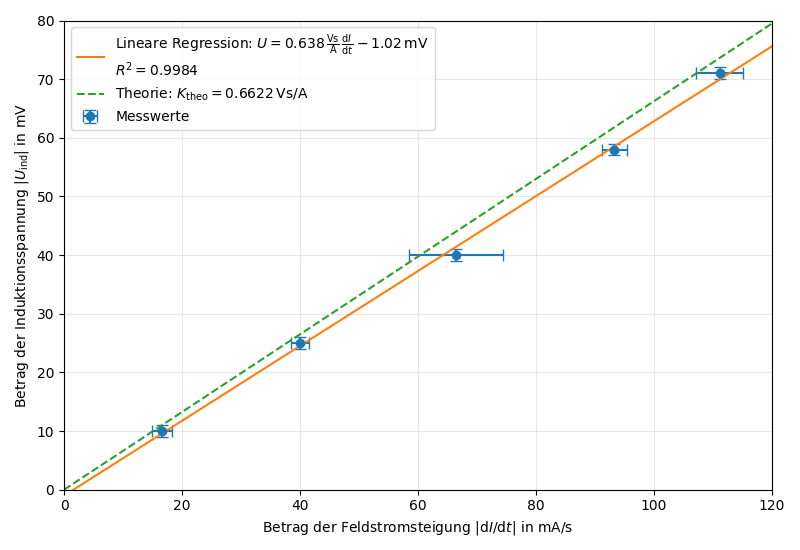
\includegraphics[width=0.8\textwidth]{Images/tv4.png}
    \caption{Induktionsspannung in Abhängigkeit von der Feldstromsteigung.}
    \label{fig:tv4}
\end{figure}


\subsection{Diskussion}
\noindent
Sowohl die Form der aufgezeichneten Kurven als auch die quantitative Auswertung
stimmen mit dem Induktionsgesetz überein. Der Feldstrom besitzt einen
dreieckförmigen Verlauf und ändert sich innerhalb einer Halbperiode
näherungsweise linear. Seine zeitliche Ableitung ist daher innerhalb einer
Halbperiode annähernd konstant. Entsprechend wurde eine näherungsweise
rechteckförmige und innerhalb einer Halbperiode konstante Induktionsspannung
beobachtet.
\noindent
Beim Wechsel von einer steigenden zu einer fallenden Flanke ändert
$\mathrm dI/\mathrm dt$ sein Vorzeichen. Gleichzeitig wechselt auch die
Induktionsspannung ihre Polarität. Damit wird auch das negative Vorzeichen des
Induktionsgesetzes qualitativ bestätigt.
\noindent
Die Auftragung von $|U_{\mathrm{ind}}|$ gegen
$|\mathrm dI/\mathrm dt|$ zeigt mit $R^2=0{,}9984$ einen nahezu linearen
Zusammenhang. Dies bestätigt die vom Induktionsgesetz vorhergesagte
Proportionalität. Zusätzlich liegt die experimentell bestimmte Steigung mit

\begin{equation}
K_{\mathrm{exp}}
=
0{,}6383\,\mathrm{\frac{Vs}{A}}
\end{equation}
\noindent
nahe am theoretischen Wert

\begin{equation}
K_{\mathrm{theo}}
=
0{,}6622\,\mathrm{\frac{Vs}{A}}.
\end{equation}
\noindent
Die relative Abweichung beträgt etwa $3{,}6\,\%$.
\noindent
Die Stärke der verwendeten Methode liegt darin, dass das Induktionsgesetz sowohl
qualitativ über die Form der Kurven als auch quantitativ über die Abhängigkeit der
Induktionsspannung von der Feldstromsteigung überprüft werden kann. Die
quantitative Genauigkeit ist jedoch insbesondere durch das manuelle Ablesen der
Kurven vom Millimeterpapier, die endliche Breite der Schreiberlinie und das
manuelle Legen der Ausgleichsgeraden begrenzt. Zusätzlich geht die Unsicherheit
des Messwiderstands in die Bestimmung des Feldstroms ein.
\noindent
Für die Fläche der Induktionsspule und die Windungszahlen lagen keine
Unsicherheitsangaben vor. Diese Beiträge konnten daher bei der Unsicherheit des
theoretischen Proportionalitätsfaktors nicht berücksichtigt werden. Ebenso wurde
keine zusätzliche Kalibrierunsicherheit des Schreibers berücksichtigt.
\noindent
Insgesamt bestätigen die beobachteten Kurvenformen, die nahezu lineare
Abhängigkeit zwischen Induktionsspannung und Feldstromsteigung sowie die geringe
Abweichung des experimentellen vom theoretischen Proportionalitätsfaktor das
Induktionsgesetz sehr gut.







\newpage
\chapter{Anhang}
\section{Python Scripts}
Die Python Scripts, die zum Plotten der Grafiken verwendet wurden, wurden teilweise mit Unterstützung von KI erstellt und dann nach den eigenen Bedürfnissen weiter
bearbeitet.
\definecolor{codegreen}{rgb}{0,0.6,0}
\definecolor{codegray}{rgb}{0.5,0.5,0.5}
\definecolor{codepurple}{rgb}{0.58,0,0.82}
\definecolor{backcolour}{rgb}{0.95,0.95,0.92}

\lstdefinestyle{python}{
    backgroundcolor=\color{backcolour},   
    commentstyle=\color{codegreen},
    keywordstyle=\color{magenta},
    numberstyle=\tiny\color{codegray},
    stringstyle=\color{codepurple},
    basicstyle=\ttfamily\footnotesize,
    breakatwhitespace=false,         
    breaklines=true,                 
    captionpos=b,                    
    keepspaces=true,                 
    numbers=left,                    
    numbersep=5pt,                  
    showspaces=false,                
    showstringspaces=false,
    showtabs=false,                  
    tabsize=2
}

\subsection{TV II:}
\subsubsection{Berechnung der Winkel}
\label{scr:calcAng}
\begin{scriptsize}
\lstset{style=python}
\begin{lstlisting}[language=python]
import numpy as np
from texttable import Texttable
from latextable import draw_latex
from math import ceil

alpha = np.array([0, 10, 20, 30, 40, 50, 60, 70, 80, 90])
_beta = np.array([268.0, 286.0, 307.0, 322.5, 340.0, 356.0, 370.5, 384.0, 396.0, 407.5])
dalpha = 2
dbeta = 1
beta = _beta - 268.0
phi = alpha - beta
dphi = np.sqrt(dalpha**2 + dbeta**2)


table = Texttable()
table.set_cols_dtype(['t', 't', 't'])
table.set_cols_align(['c', 'c', 'c'])
table.add_row(['$\\alpha$ in $^{\\circ}$', '$\\beta$ in $^{\\circ}$', '$\\varphi$ in $^{\\circ}$'])
for i in range(len(alpha)):
    table.add_row([f"${alpha[i]:.1f} \pm {ceil(dalpha * 10) / 10:.1f}$", f"${beta[i]:.1f} \pm {ceil(dbeta * 10) / 10:.1f}$", f"${phi[i]:.1f} \pm {ceil(dphi * 10) / 10:.1f}$"])

latex_table = draw_latex(table, caption="Berechnete Winkel", label="tab:angles")
print(latex_table)

print("\nBerechnete Winkel:")
print(f"alpha = np.array({alpha})")
print(f"phi = np.array({phi})")
\end{lstlisting}
\end{scriptsize}

\subsubsection{Plot des $\phi$-$\sin(\alpha)$-Diagramms}
\label{scr:phiSinAlpha}
\begin{scriptsize}
\lstset{style=python}
\begin{lstlisting}[language=python]
import numpy as np
import matplotlib.pyplot as plt
from math import ceil

alpha = np.array([0, 10, 20, 30, 40, 50, 60, 70, 80, 90])
sinAlpha = np.sin(np.radians(alpha))
phi = -np.array([0.0, -8.0, -19.0, -24.5, -32.0, -38.0, -42.5, -46.0, -48.0, -49.5])
dphi = 2.3

line, cov = np.polyfit(sinAlpha, phi, 1, cov=True)
slope, intercept = line
d_slope, d_intercept = np.sqrt(np.diag(cov)) #Berechnung der Fehler der Fitparameter

y_line = np.polyval(line, sinAlpha)
slope, intercept = line
label_fit = (rf"Linearer Fit $\varphi = a \cdot \sin(\alpha) + b$" "\n" rf"mit $a = {slope:.1f} \pm {ceil(d_slope*10)/10:.1f}, b = {intercept:.1f} \pm {ceil(d_intercept*10)/10:.1f}$")

fig, ax = plt.subplots(figsize=(7, 4.5))

ax.errorbar(
    sinAlpha, phi,
    yerr=dphi,
    fmt='o',
    ms=4,
    color='steelblue',
    mec='white',
    mew=0.8,
    ecolor='steelblue',
    elinewidth=1,
    capsize=4,
    capthick=1,
    label="Messwerte",
    zorder=3,
)

ax.plot(
    sinAlpha, y_line,
    color='tomato',
    linewidth=1.5,
    linestyle='--',
    label=label_fit,
    zorder=2,
)

# Achsen bei 0,0
ax.spines['left'].set_position('zero')
ax.spines['bottom'].set_position('zero')
ax.spines['right'].set_visible(False)
ax.spines['top'].set_visible(False)

# Achsenpfeile
ax.plot(1, 0, ">k", transform=ax.get_yaxis_transform(), clip_on=False, ms=4)
ax.plot(0, 1, "^k", transform=ax.get_xaxis_transform(), clip_on=False, ms=4)

ax.set_xlim(-0.05, 1.1)
ax.set_ylim(-5, 60)

ax.set_xlabel(r"$\sin(\alpha)$", labelpad=15)
ax.set_ylabel(r"$\varphi$ in $^{\circ}$", labelpad=15, rotation=0, ha='right')

ax.set_title(r"$\varphi$ in Abhaengigkeit von $\sin(\alpha)$", pad=12, fontsize=12)
ax.grid(True, linestyle=':', alpha=0.4, color='gray')

ax.legend(
    loc='upper left',
    framealpha=0.9,
    edgecolor='lightgray',
    fontsize=9,
)

plt.tight_layout()
plt.savefig("./03_MAG/Images/PhiSinAlpha.png", dpi=800)
plt.show()
\end{lstlisting}
\end{scriptsize}

\subsection{TV III:}
\subsubsection{Berechnung des Mittelwerts der Spannungsamplituden}
\label{scr:meanAndError}
\begin{scriptsize}
\lstset{style=python}
\begin{lstlisting}[language=python]
import numpy as np

values = [1.095, 1.105, 1.055, 1.125, 1.085, 1.125, 1.080, 
          1.125, 1.120, 1.130, 1.095, 1.135, 1.115, 1.115, 
          1.080, 1.115]

mean = np.mean(values)
mean = np.round(mean, 3)
sigma = np.std(values, ddof = 1) #Standardabweichung einer Stichprobe mit Besselscher Korrektur
error = sigma / np.sqrt(len(values))
error = np.round(error, 3)
print(f"\hat{{U}}_{{\mathrm{{ind}}}} = {mean} \pm {error}")
\end{lstlisting}
\end{scriptsize}


\subsubsection{Python-Code zur Auswertung des Induktionsgesetzes}
\label{scr:induktionsgesetz}

\begin{scriptsize}
\lstset{style=python}
\begin{lstlisting}[language=python]
import numpy as np
import matplotlib.pyplot as plt

# Folgende Arrays enthalten die Messwerte

# Feldstromsteigungen in mA/s
dIdt = np.array([
    16.625,
    40.000,
    66.500,
    93.300,
    111.1667
])

# Unsicherheiten der Feldstromsteigungen in mA/s
dIdt_err = np.array([
    1.7,
    1.5,
    8.0,
    2.1,
    4.0
])

# Induktionsspannungen in mV
U_ind = np.array([
    10.0,
    25.0,
    40.0,
    58.0,
    71.0
])

# Ableseunsicherheit der Induktionsspannung in mV
U_err = np.ones(len(U_ind)) * 1.0


# Lineare Regression
m_exp, b_exp = np.polyfit(dIdt, U_ind, 1)

# Vorhergesagte Werte zur Berechnung von R^2
U_fit = m_exp * dIdt + b_exp

ss_res = np.sum((U_ind - U_fit)**2)
ss_tot = np.sum((U_ind - np.mean(U_ind))**2)

R2 = 1 - ss_res / ss_tot


# Theoretischer Proportionalitaetsfaktor
# K_theo = 0.6622 Vs/A
#
# Da auf der x-Achse mA/s und auf der y-Achse mV
# verwendet werden, besitzt die theoretische Gerade
# numerisch dieselbe Steigung.

K_theo = 0.6622


# Werte fuer die Geraden
x = np.linspace(0, 120, 500)

y_exp = m_exp * x + b_exp
y_theo = K_theo * x


# Diagramm
plt.figure(figsize=(8, 5.5))

# Messwerte mit horizontalen und vertikalen Fehlerbalken
plt.errorbar(
    dIdt,
    U_ind,
    xerr=dIdt_err,
    yerr=U_err,
    fmt='o',
    capsize=4,
    label='Messwerte'
)

# Experimentelle Ausgleichsgerade
plt.plot(
    x,
    y_exp,
    label=(
        rf'Lineare Regression: '
        rf'$U = {m_exp:.3f}\,\frac{{\mathrm{{Vs}}}}{{\mathrm{{A}}}}'
        rf'\,\frac{{\mathrm{{d}}I}}{{\mathrm{{d}}t}}'
        rf'{b_exp:+.2f}\,\mathrm{{mV}}$'
        '\n'
        rf'$R^2={R2:.4f}$'
    )
)

# Theoretisch erwartete Gerade
plt.plot(
    x,
    y_theo,
    '--',
    label=(
        rf'Theorie: '
        rf'$K_\mathrm{{theo}}={K_theo:.4f}\,\mathrm{{Vs/A}}$'
    )
)

plt.xlabel(
    r'Betrag der Feldstromsteigung '
    r'$|\mathrm{d}I/\mathrm{d}t|$ in $\mathrm{mA/s}$'
)

plt.ylabel(
    r'Betrag der Induktionsspannung '
    r'$|U_{\mathrm{ind}}|$ in $\mathrm{mV}$'
)

plt.xlim(0, 120)
plt.ylim(0, 80)

plt.grid(alpha=0.3)
plt.legend()
plt.tight_layout()

# Optionales Speichern der Abbildung
# plt.savefig(
#     "induktionsgesetz_tv4.pdf",
#     bbox_inches="tight"
# )

plt.show()


# Ausgabe der Ergebnisse
print(
    f"Experimentelle Steigung: "
    f"K_exp = {m_exp:.4f} Vs/A"
)

print(
    f"Achsenabschnitt: "
    f"b = {b_exp:.2f} mV"
)

print(
    f"Bestimmtheitsmass: "
    f"R^2 = {R2:.4f}"
)

print(
    f"Theoretische Steigung: "
    f"K_theo = {K_theo:.4f} Vs/A"
)

abweichung = abs(m_exp - K_theo) / K_theo * 100

print(
    f"Relative Abweichung: "
    f"{abweichung:.1f} %"
)
\end{lstlisting}
\end{scriptsize}

\end{document}
